\documentclass{article}

\usepackage{minted}
\usepackage{xcolor}
\usepackage{graphicx}

\usepackage{booktabs}
\usepackage{tabularx}
\usepackage{siunitx}
\usepackage{hyperref}

\title{EE 450 Wireshark Lab: TCP Report}
\author{Shangning Xu}

\begin{document}

\maketitle
\newpage

\begin{abstract}
    We answer assigned questions in this report for the Wireshark Lab: TCP, with the experiment performed in the university-wide network ``USC Secure Wireless'' under macOS 12.2.1 with Wireshark 3.6.2 and HTTP requests sent by Safari 15.3.
\end{abstract}

\section{Answers to Questions}

\begin{enumerate}
    \item The client IP address is 192.168.1.102 and port number 1161, as shown below for the POST request:
\begin{minted}[breaklines, escapeinside=!!]{text}
Internet Protocol Version 4, Src: !\colorbox{yellow}{192.168.1.102}!, Dst: 128.119.245.12
Transmission Control Protocol, Src Port: !\colorbox{yellow}{1161}!, Dst Port: 80, Seq: 164041, Ack: 1, Len: 50
\end{minted}

    \item As shown above, The IP address of gaia.cs.umass.edu is 128.119.245.12 and the port number is 80.
    
    \item In my own trace, the IP address and TCP port number used by the client computer are 10.26.97.213 and 53397, respectively.
\begin{minted}[breaklines, escapeinside=!!]{text}
Internet Protocol Version 4, Src: !\colorbox{yellow}{10.26.97.213}!, Dst: 128.119.245.12
Transmission Control Protocol, Src Port: !\colorbox{yellow}{53397}!, Dst Port: 80, Seq: 151893, Ack: 1, Len: 1044
\end{minted}
    
    \item The sequence number of the SYN segment is 601204107 as shown below. The SYN bit identifies the segment as a SYN segment.
\begin{minted}[breaklines, escapeinside=!!]{text}
53397 → 80 [SYN] Seq=!\colorbox{yellow}{601204107}! Win=65535 Len=0 MSS=1460 WS=64 TSval=3399580464 TSecr=0 SACK_PERM=1
\end{minted}

    For tcp-ethereal-trace-1, the sequence number of the SYN segment is 232129012.

    \item As shown below, the sequence number of the SYNACK segment is 948975578 and the value of the Acknowledgement field is 601204108, which is determined by adding 1 to the sequence number of the SYN segment. The SYN and ACK bits identifies the segment as a SYNACK segment.
\begin{minted}[breaklines, escapeinside=!!]{text}
80 → 53397 [SYN, ACK] Seq=!\colorbox{yellow}{948975578}! Ack=!\colorbox{yellow}{601204108}! Win=28960 Len=0 MSS=1386 SACK_PERM=1 TSval=1064245001 TSecr=3399580464 WS=128
\end{minted}

    For tcp-ethereal-trace-1, the sequence number of the SYNACK segment is 883061785 and the value of the Acknowledgement field is 232129013.

    \item The sequence number of the TCP segment containing the HTTP POST command is 601204108 as shown below.
\begin{minted}[breaklines, escapeinside=!!]{text}
53397 → 80 [PSH, ACK] Seq=!\colorbox{yellow}{601204108}! Ack=948975579 Win=131904 Len=615 TSval=3399580531 TSecr=1064245001
\end{minted}

    For tcp-ethereal-trace-1, the sequence number of the TCP segment containing the HTTP POST command is 601204108 and the value of the Acknowledgement field is 883061785.

    \item All answers to this question are shown in Table~\ref{tab:six-segments} for our own collected traces and Table~\ref{tab:tcp-ethereal-trace-1-six-segments} for tcp-ethereal-trace-1.

    \begin{table}[tb]
        \centering
        \caption{First six TCP segments (in the first table) and their acknowledgments (in the second table) in the POST request, starting at the segment that contains the POST request.}
        \label{tab:six-segments}

        \vspace{2ex}
        
        \begin{tabular}{@{}rrrrrrr@{}}
            \toprule
            No. & Time & Length & Seq Num & \begin{tabular}{@{}c@{}} ACK \\ No.\end{tabular} & \begin{tabular}{@{}c@{}} RTT \\ /ms \end{tabular} & \begin{tabular}{@{}c@{}} \texttt{EstimatedRTT} \\ /ms \end{tabular} \\ \midrule
            31 & 6.324287 & 615 & 601204108 & 42 & 66.164 & 66.164 \\
            32 & 6.324856 & 137 & 601204723 & 43 & 65.602 & 66.094 \\
            33 & 6.326497 & 1374 & 601204860 & 44 & 63.962 & 65.828 \\
            34 & 6.326498 & 1374 & 601206234 & 44 & 63.961 & 65.595 \\
            35 & 6.326500 & 1374 & 601207608 & 50 & 64.876 & 65.505 \\
            36 & 6.326500 & 1374 & 601208982 & 50 & 64.876 & 65.426 \\ \bottomrule
        \end{tabular}

        \vspace{2ex}

        \begin{tabularx}{\linewidth}{@{}ll>{\raggedright\arraybackslash}X@{}}
            \toprule
            No. & Time & Info \\ \midrule
            42 & 6.390451 & 80  \textgreater  53397 {[}ACK{]} Seq=948975579 Ack=601204723 Win=30208 Len=0 TSval=1064245069 TSecr=3399580531 \\
            43 & 6.390458 & 80  \textgreater  53397 {[}ACK{]} Seq=948975579 Ack=601204860 Win=31488 Len=0 TSval=1064245070 TSecr=3399580532 \\
            44 & 6.390459 & 80  \textgreater  53397 {[}ACK{]} Seq=948975579 Ack=601207608 Win=36992 Len=0 TSval=1064245071 TSecr=3399580534 \\
            50 & 6.391376 & 80  \textgreater  53397 {[}ACK{]} Seq=948975579 Ack=601214478 Win=50688 Len=0 TSval=1064245072 TSecr=3399580534 \\ \bottomrule
        \end{tabularx}
    \end{table}
    
    \begin{table}[htb]
        \caption{First six TCP segments in the POST request in tcp-ethereal-trace-1, starting at the segment that contains the POST request.}
        \label{tab:tcp-ethereal-trace-1-six-segments}
        \medskip
        \begin{tabular}{@{}rrrrrrr@{}}
            \toprule
            No. & Time & Seq Num & Length & \begin{tabular}[c]{@{}c@{}}ACK\\ Time\end{tabular} & \begin{tabular}[c]{@{}c@{}}RTT\\ /ms\end{tabular} & \begin{tabular}[c]{@{}c@{}}\texttt{EstimatedRTT}\\ /ms\end{tabular} \\ \midrule
            4 & 0.026477 & 232129013 & 565 & 0.053937 & 27.460 & 27.460 \\
            5 & 0.041737 & 232129578 & 1460 & 0.077294 & 35.557 & 28.472 \\
            7 & 0.054026 & 232131038 & 1460 & 0.124085 & 70.059 & 33.670 \\
            8 & 0.054690 & 232132498 & 1460 & 0.169118 & 114.428 & 43.764 \\
            10 & 0.077405 & 232133958 & 1460 & 0.217299 & 139.894 & 55.780 \\
            11 & 0.078157 & 232135418 & 1460 & 0.267802 & 189.645 & 72.513 \\ \bottomrule
        \end{tabular}
    \end{table}
        
    \item The length of each of the first six TCP segments is shown in Table~\ref{tab:six-segments} and Table~\ref{tab:tcp-ethereal-trace-1-six-segments}.

    \item The minimum amount of available buffer space is \SI{28960}{B}, advertized in the SYNACK segment sent by the server whose Wireshark ``Info'' column is provided in the answer to Question 5. This is the minimum because the receive window size kept increasing during the entire TCP connection, as observed in the Window Scaling graph in Figure~\ref{fig:our-traces}.
    
    The sender was never throttled due to lack of space in the receiver's buffer. Figure~\ref{fig:our-traces} shows that the receive window is always almost twice the number of bytes sent but not acknowledged. That is, the receiver's buffer is always nearly half empty.

    For tcp-ethereal-trace-1, the minimum amount of available buffer space is \SI{5840}{B} and the sender was never throttled.
    
    \begin{figure}[tb]
        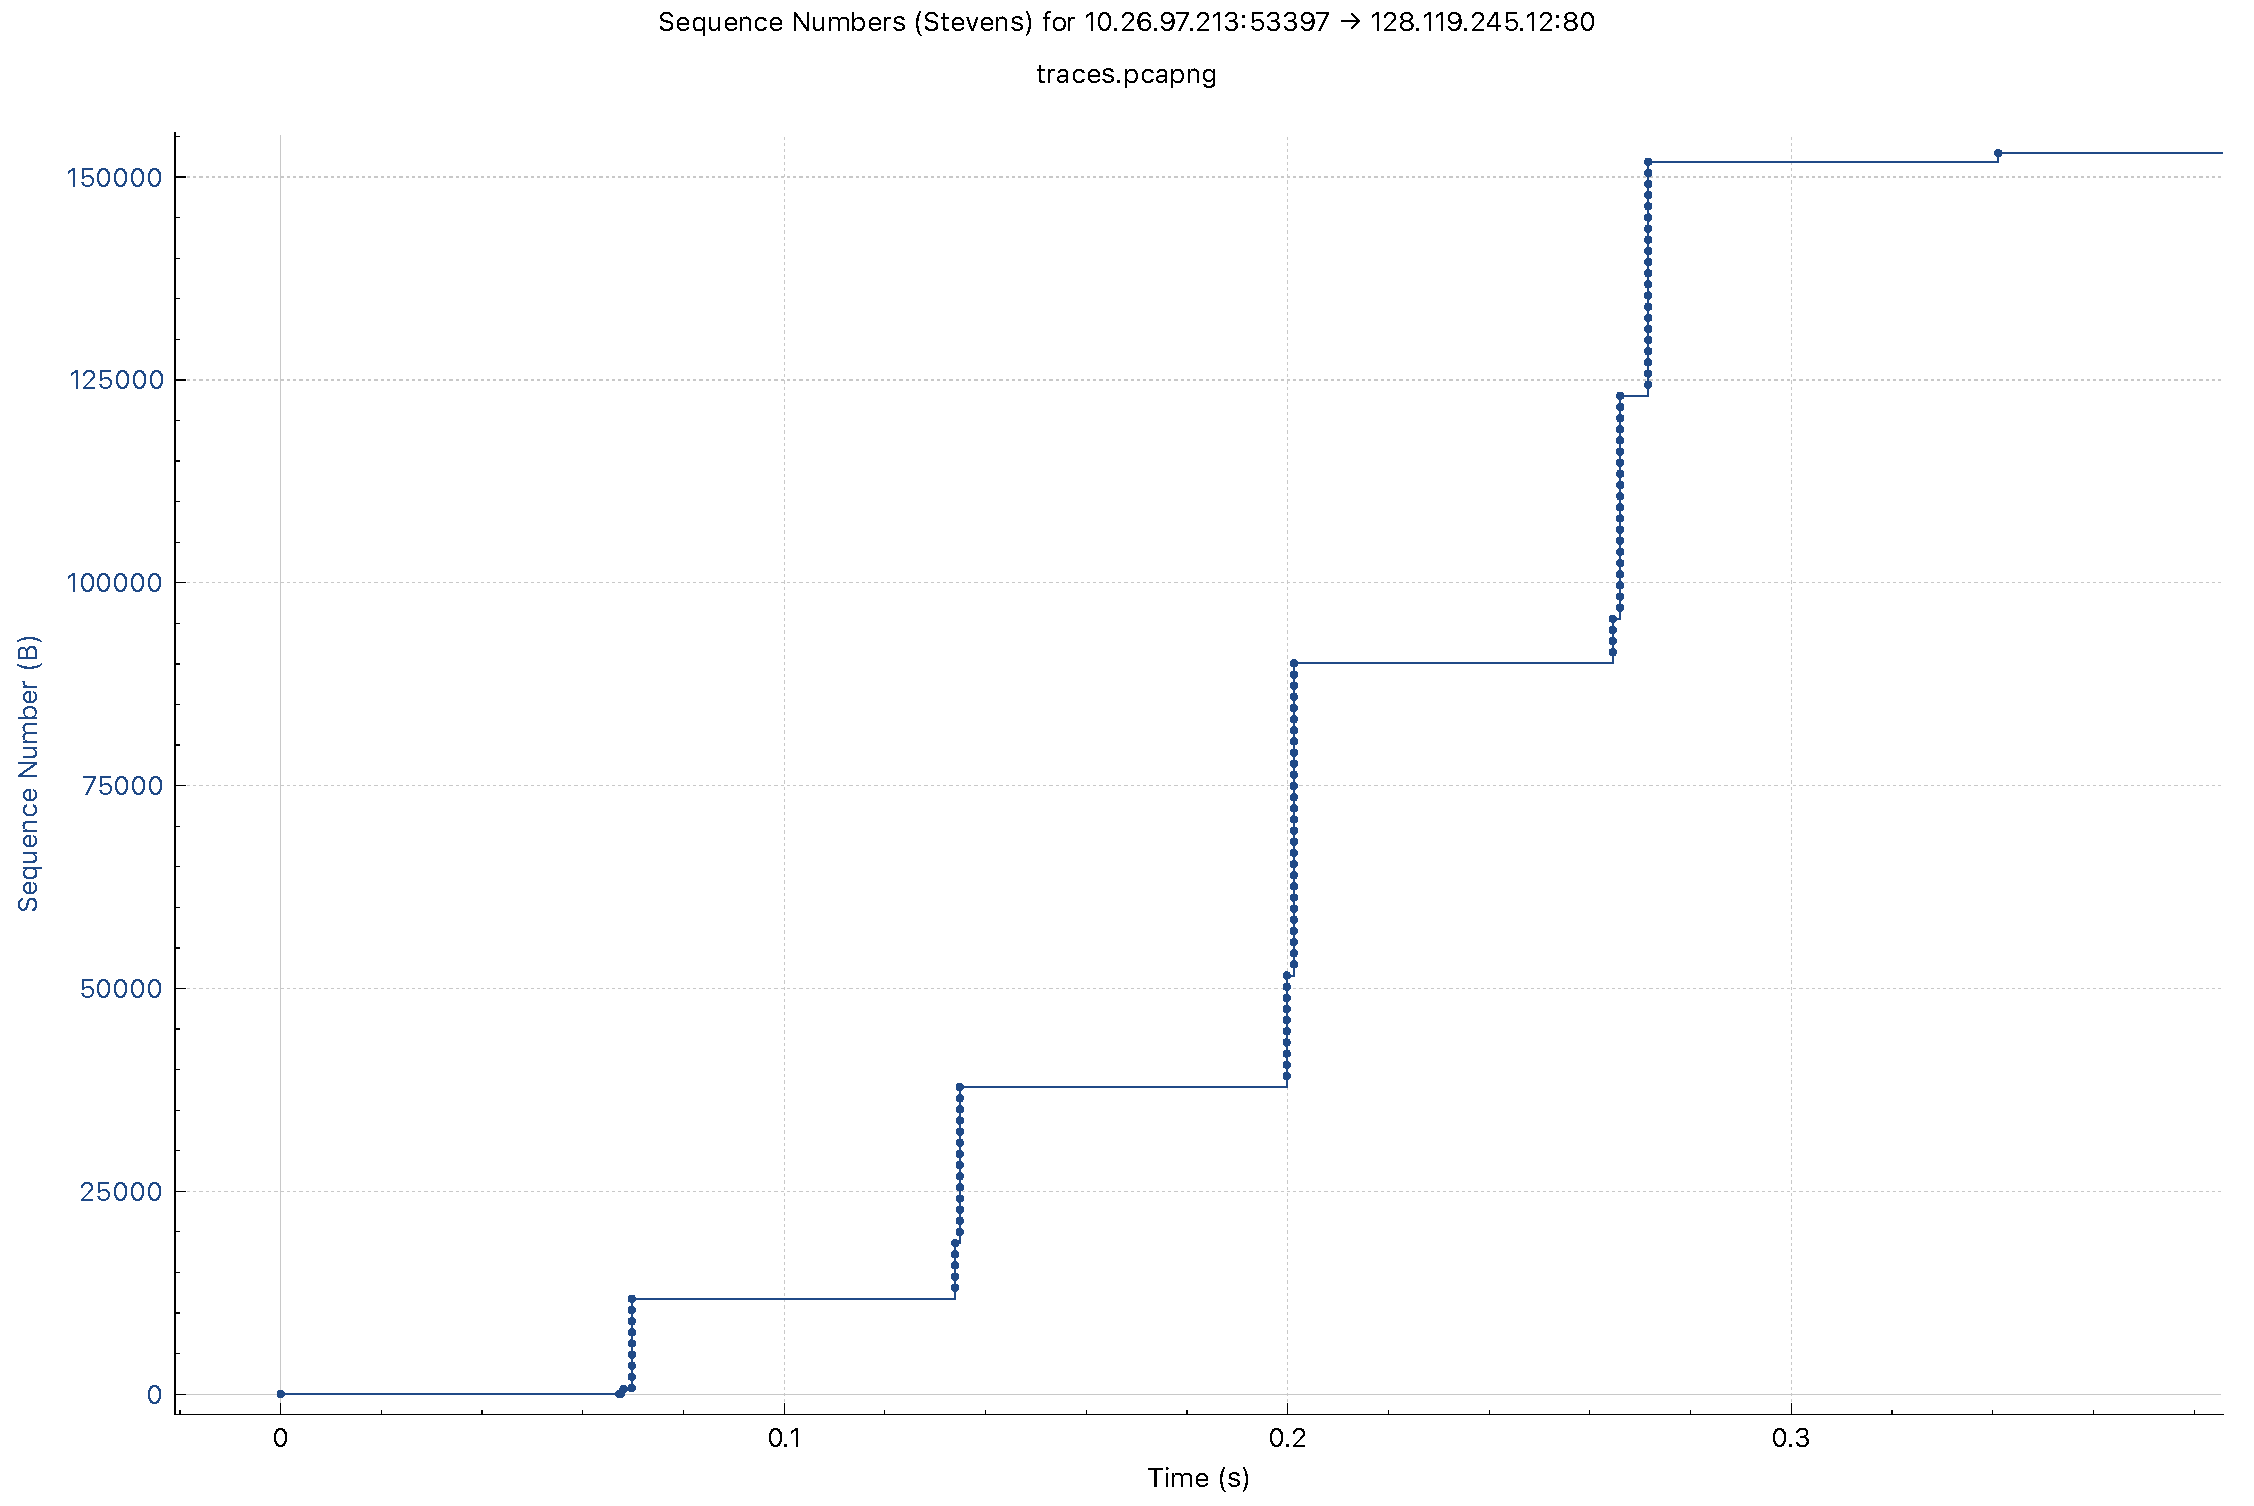
\includegraphics[width=0.49\linewidth]{img/time-sequence-stevens.pdf}
        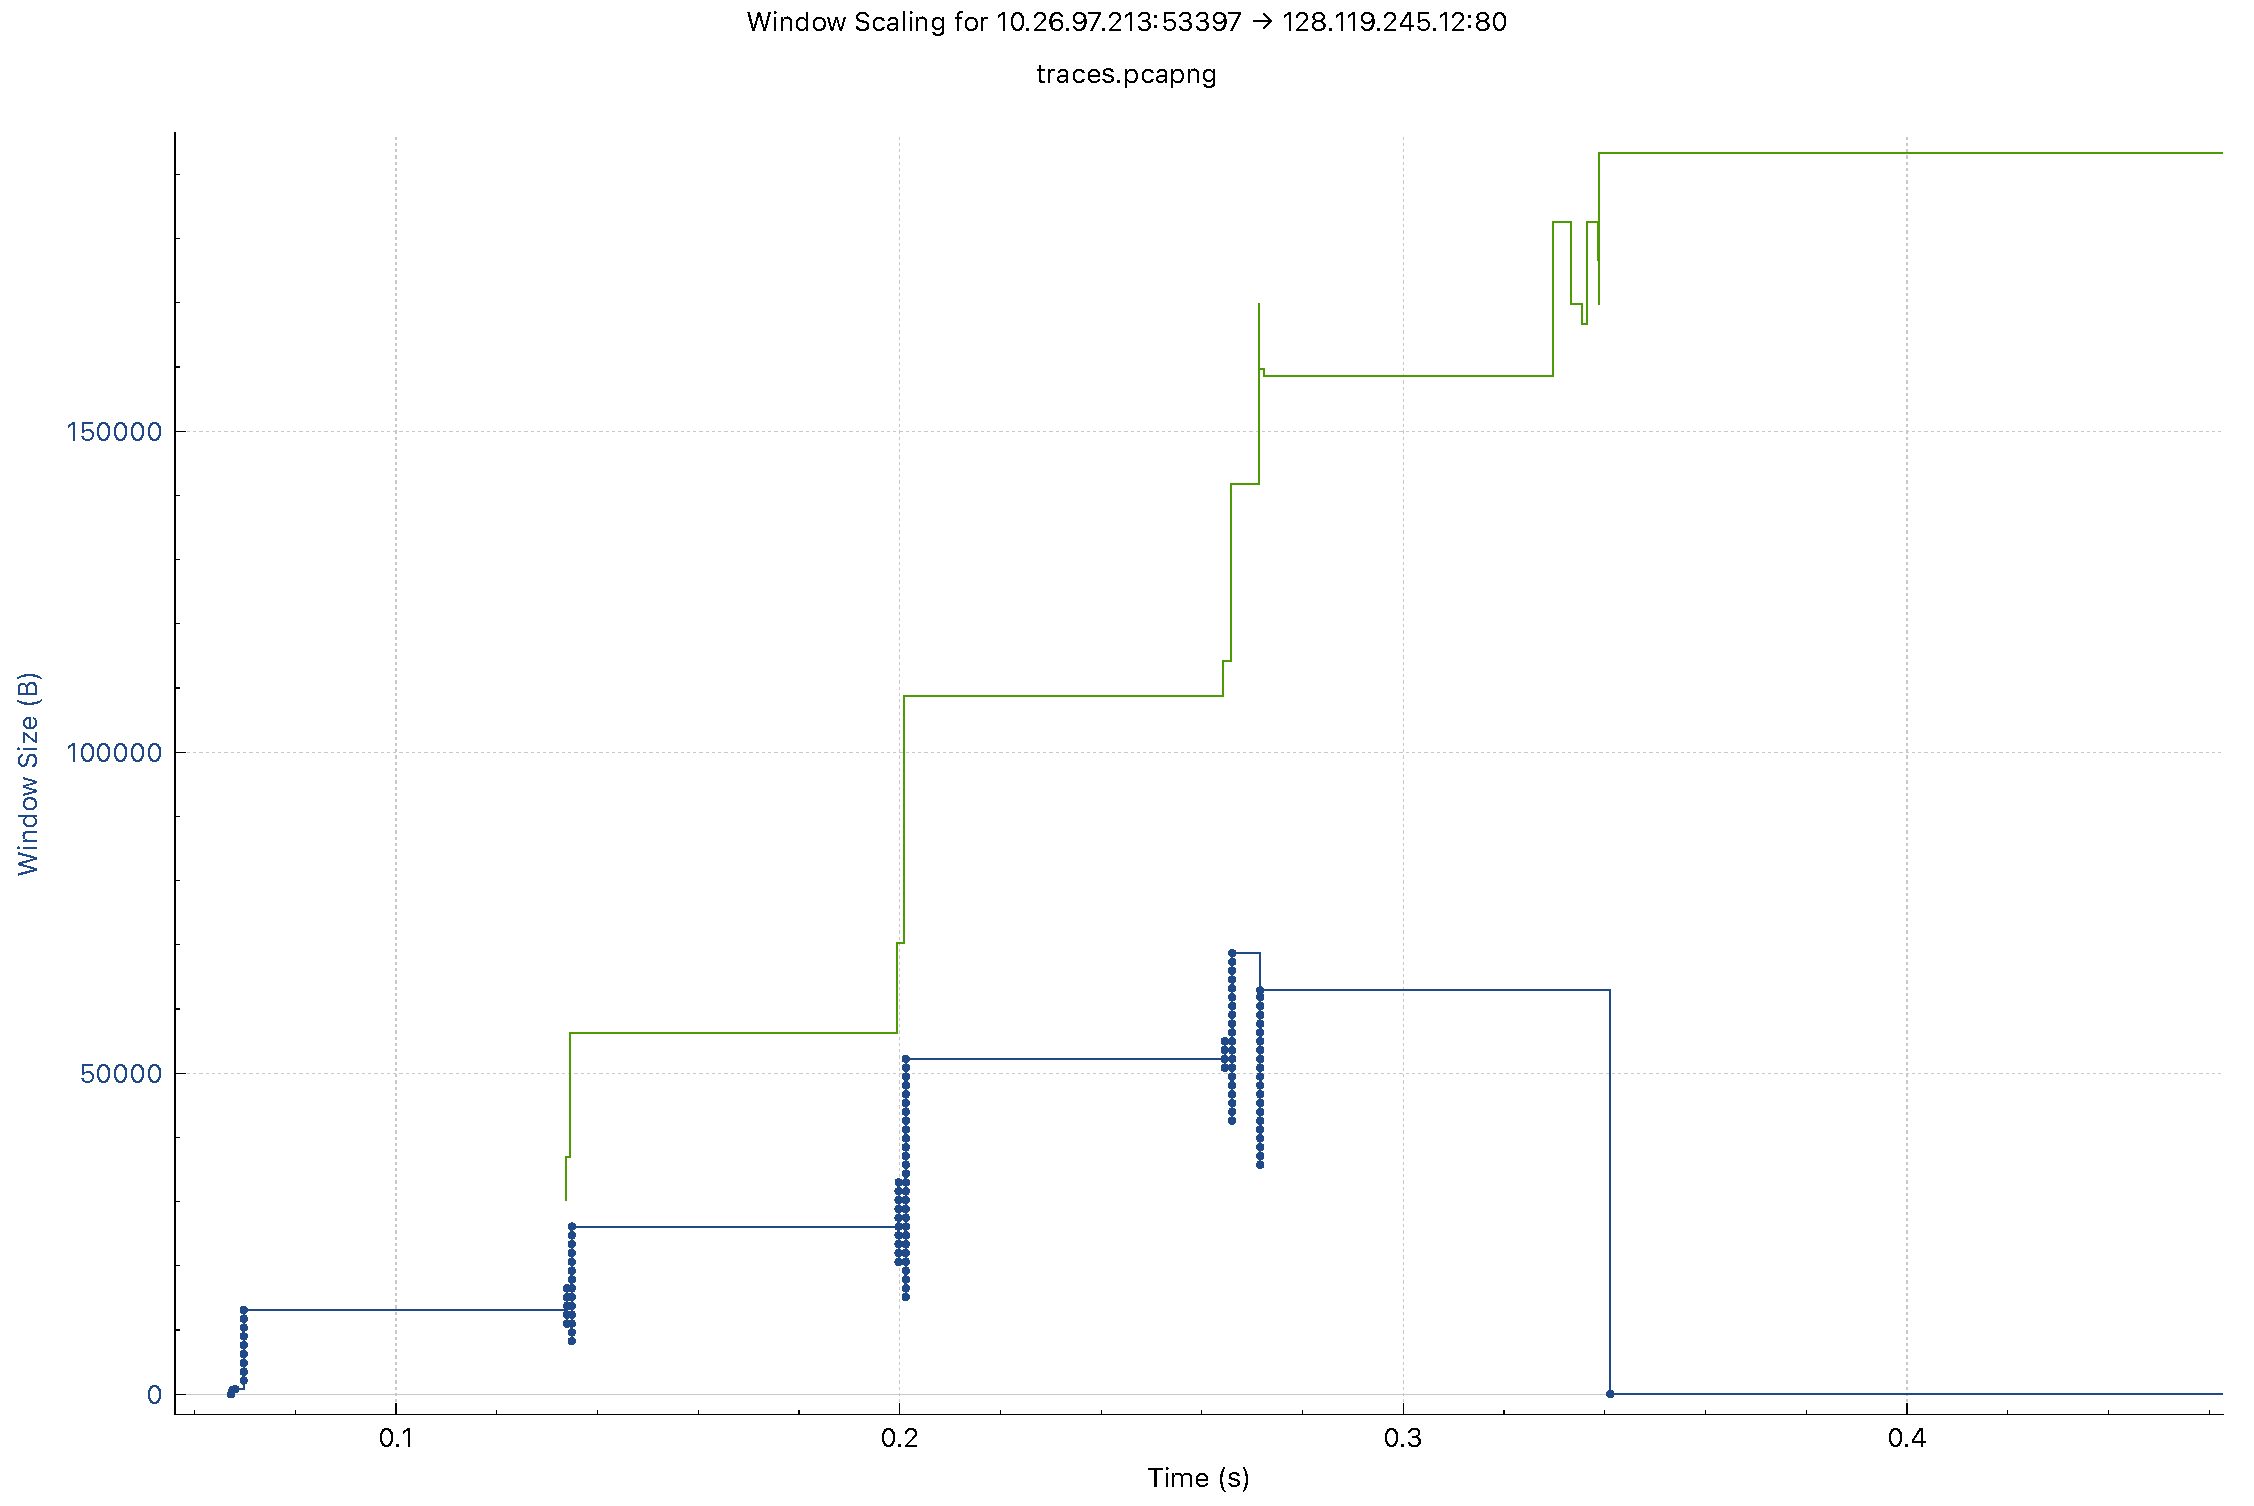
\includegraphics[width=0.49\linewidth]{img/window-scaling.pdf}
        \caption{Time Sequence (Stevens) (left) and Window Scaling (right) graph in the direction from the client to the HTTP server plotted by Wireshark for the entire TCP connection in our own traces.}
        \label{fig:our-traces}
    \end{figure}

    \item There is no retransmitted segment in either our own traces or tcp-ethereal-trace-1. I checked the \href{https://www.wireshark.org/docs/wsug_html_chunked/ChAdvTCPAnalysis.html}{TCP Analysis packet detail item} for each TCP segment to see if Wireshark labeled it as a retransmission.

    \item The amount of data acknowledged in an ACK varies from more than \SI{600}{B} (for the segment that contains the POST command and headers) to a little over \SI{10000}{B} and is typically three to five thousand bytes.
    
    We do identify a case where the receiver is ACKing every other received segment, hinting delayed ACK at play. These acknowledgments are shown below, where the difference between neighboring ACK numbers is always 2748, which is exactly twice the size of a TCP segment (\SI{1374}{B}) sent by the client.
\begin{minted}[breaklines]{text}
No.     Info
    161 80 → 53397 [ACK] Seq=1 Ack=91437 Win=158592 Len=0 TSval=1064245207 TSecr=3399580665
    162 80 → 53397 [ACK] Seq=1 Ack=94185 Win=182528 Len=0 TSval=1064245265 TSecr=3399580728
    163 80 → 53397 [ACK] Seq=1 Ack=96933 Win=182528 Len=0 TSval=1064245266 TSecr=3399580728
    164 80 → 53397 [ACK] Seq=1 Ack=99681 Win=182528 Len=0 TSval=1064245267 TSecr=3399580730
\end{minted}

    For tcp-ethereal-trace-1, typically one or two segments (\SIrange{1460}{2920}{B}) are acknowledged in an ACK. The receiver did sometimes acknowledged every other received segment, for example six segments numbered 63--68 in the trace file were acknowledged by three ACKs numbered 69--71.

    \item The throughput is
    \[
        \frac{\num{601357044} - \num{601204108}}{\SI{5.434462}{s}} = \SI{28141.88}{B/s},
    \]
    where
    \begin{itemize}
        \item the time is read from the first and the last packet in the TCP connection (note that the question asks for the throughput of the TCP connection, rather than just the throughput of the POST request),
        \item \num{601357044} is the sequence number of the FIN segment sent from the client to the server, and
        \item \num{601204108} is the sequence number of the last ACK in the three-way handshake, sent from the client to the server.
    \end{itemize}

    For tcp-ethereal-trace-1, the throughput is
    \[
        \frac{\num{232293103} - \num{232129013}}{\SI{5.651141}{s}} = \SI{29036.61}{B/s}.
    \]
    
    \item The slow start phase starts at \SI{0}{s} and ends before \SI{0.2}{s}, after which congestion avoidance takes over, as shown in the Time Sequence (Stevens) graph in Figure~\ref{fig:tcp-ethereal-trace}.
    
    The behaviors in tcp-ethereal-trace-1 differs from idealized TCP behaviors in that during the congestion avoidance phase, the number of outstanding bytes during each RTT is almost constant,  as shown in the Window Scaling graph in Figure~\ref{fig:tcp-ethereal-trace}, despite large receive window size and absence of packet loss.
    
    \begin{figure}[tb]
        \centering
        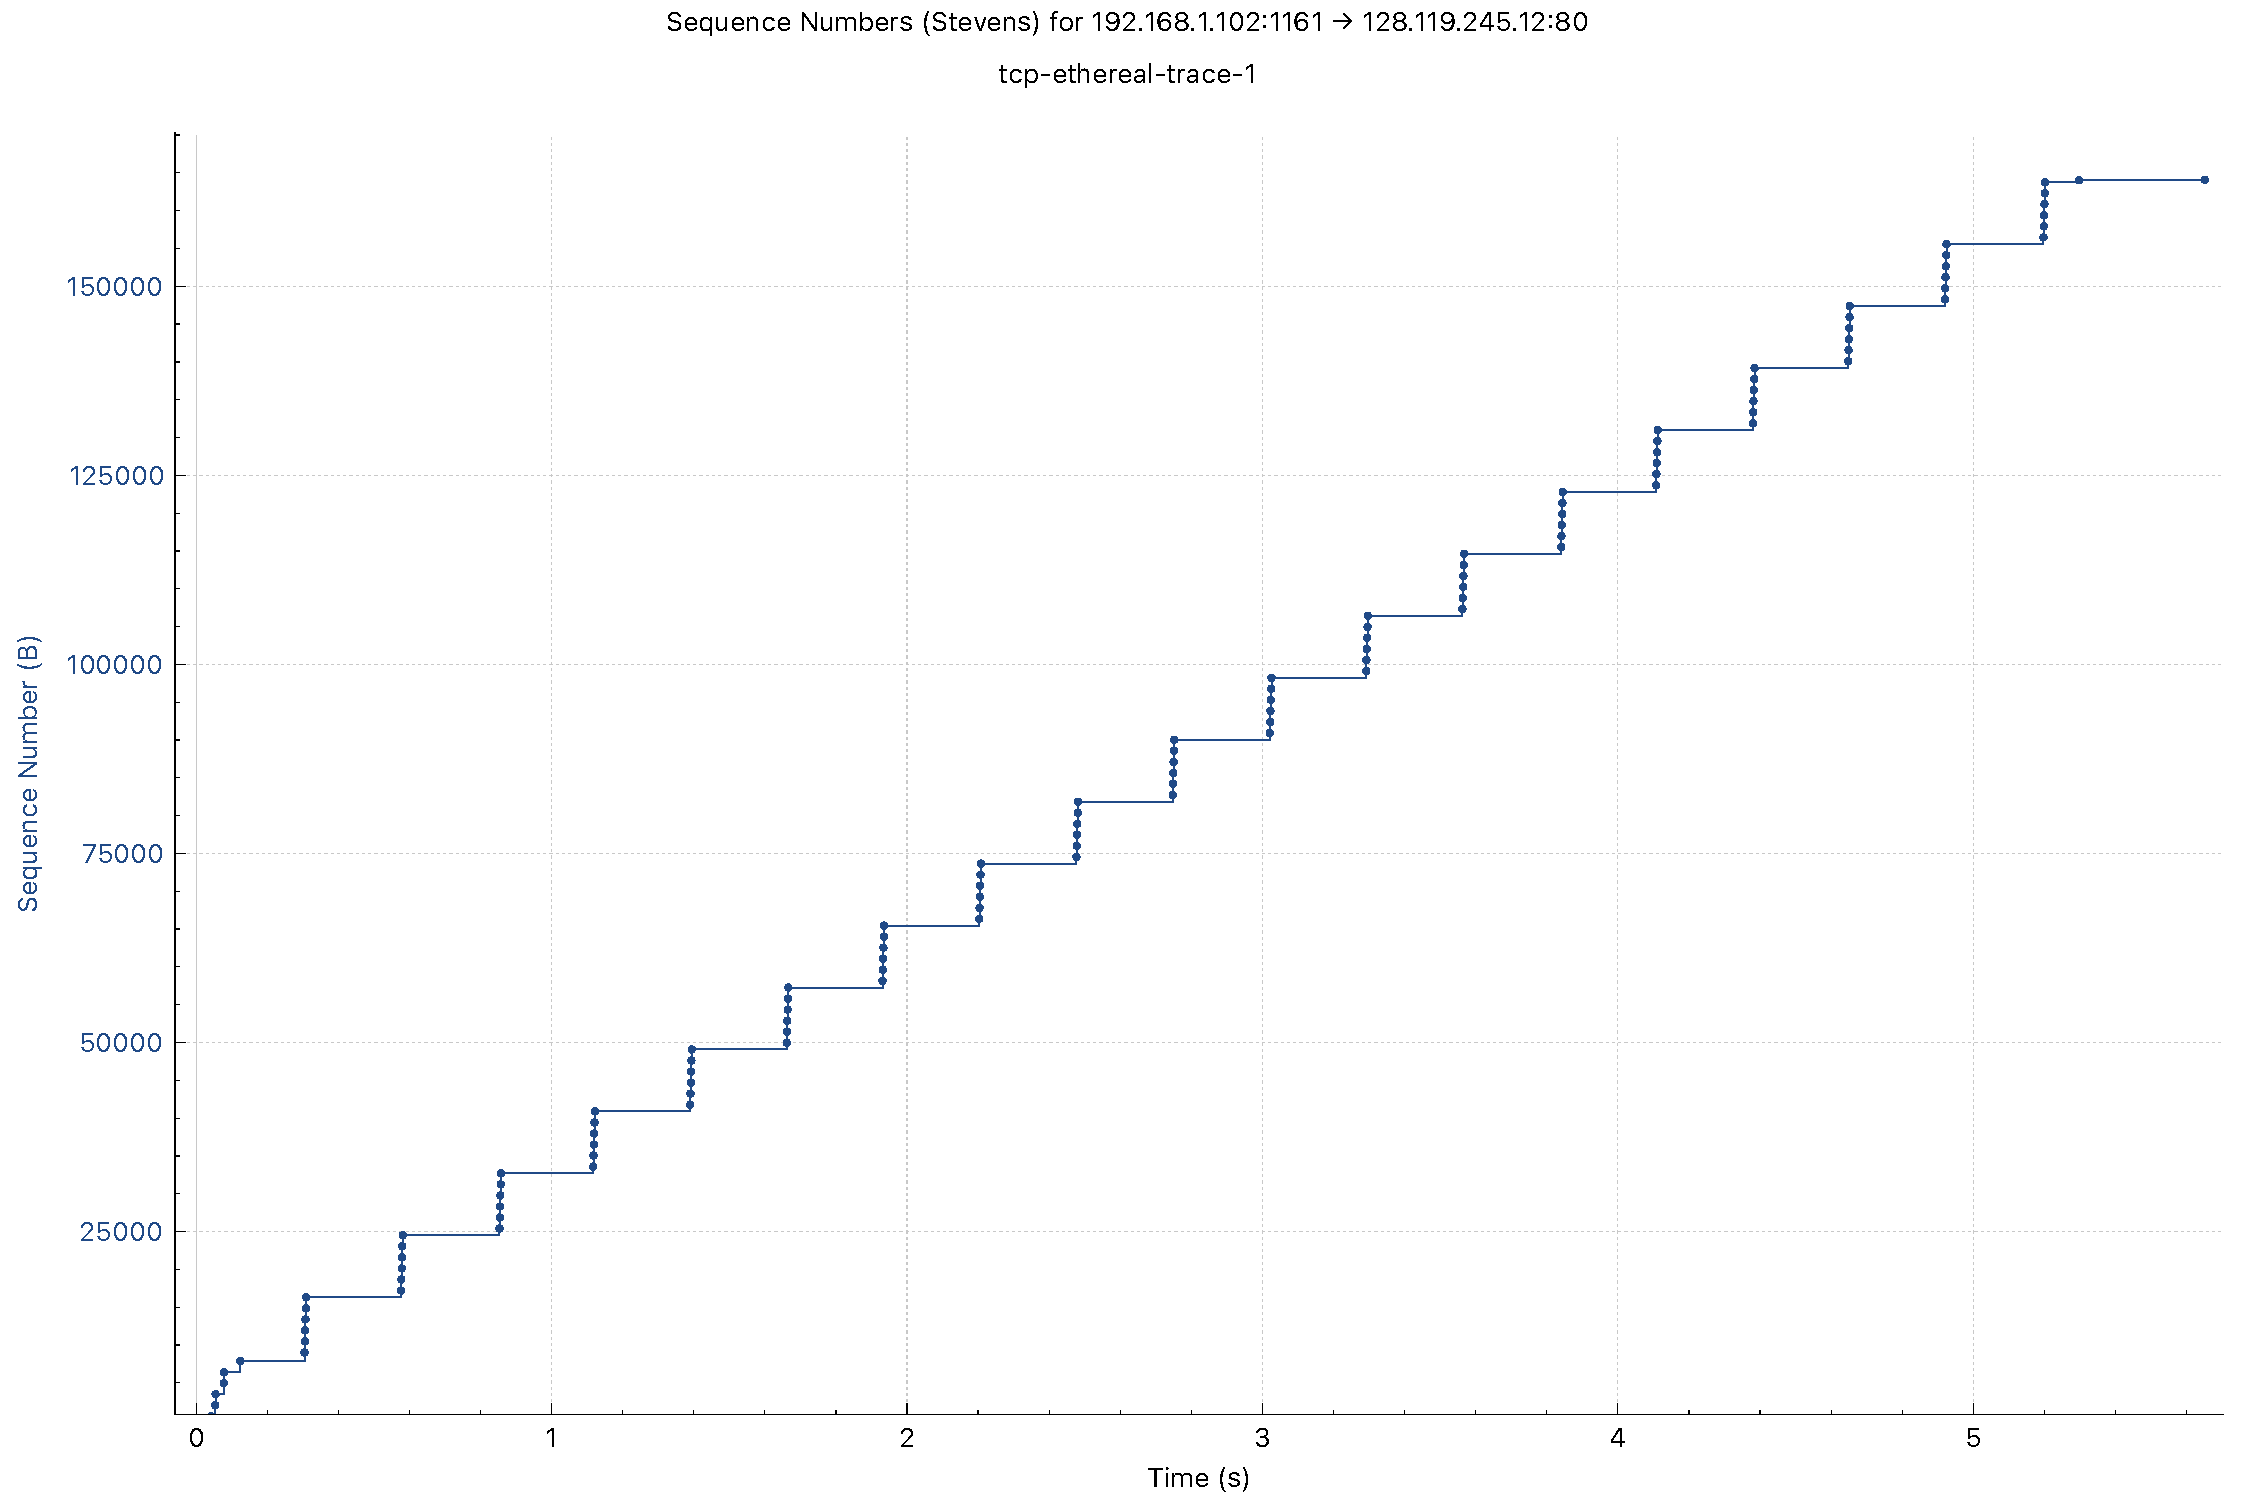
\includegraphics[width=0.49\linewidth]{img/tcp-ethereal-trace-time-sequence.pdf}
        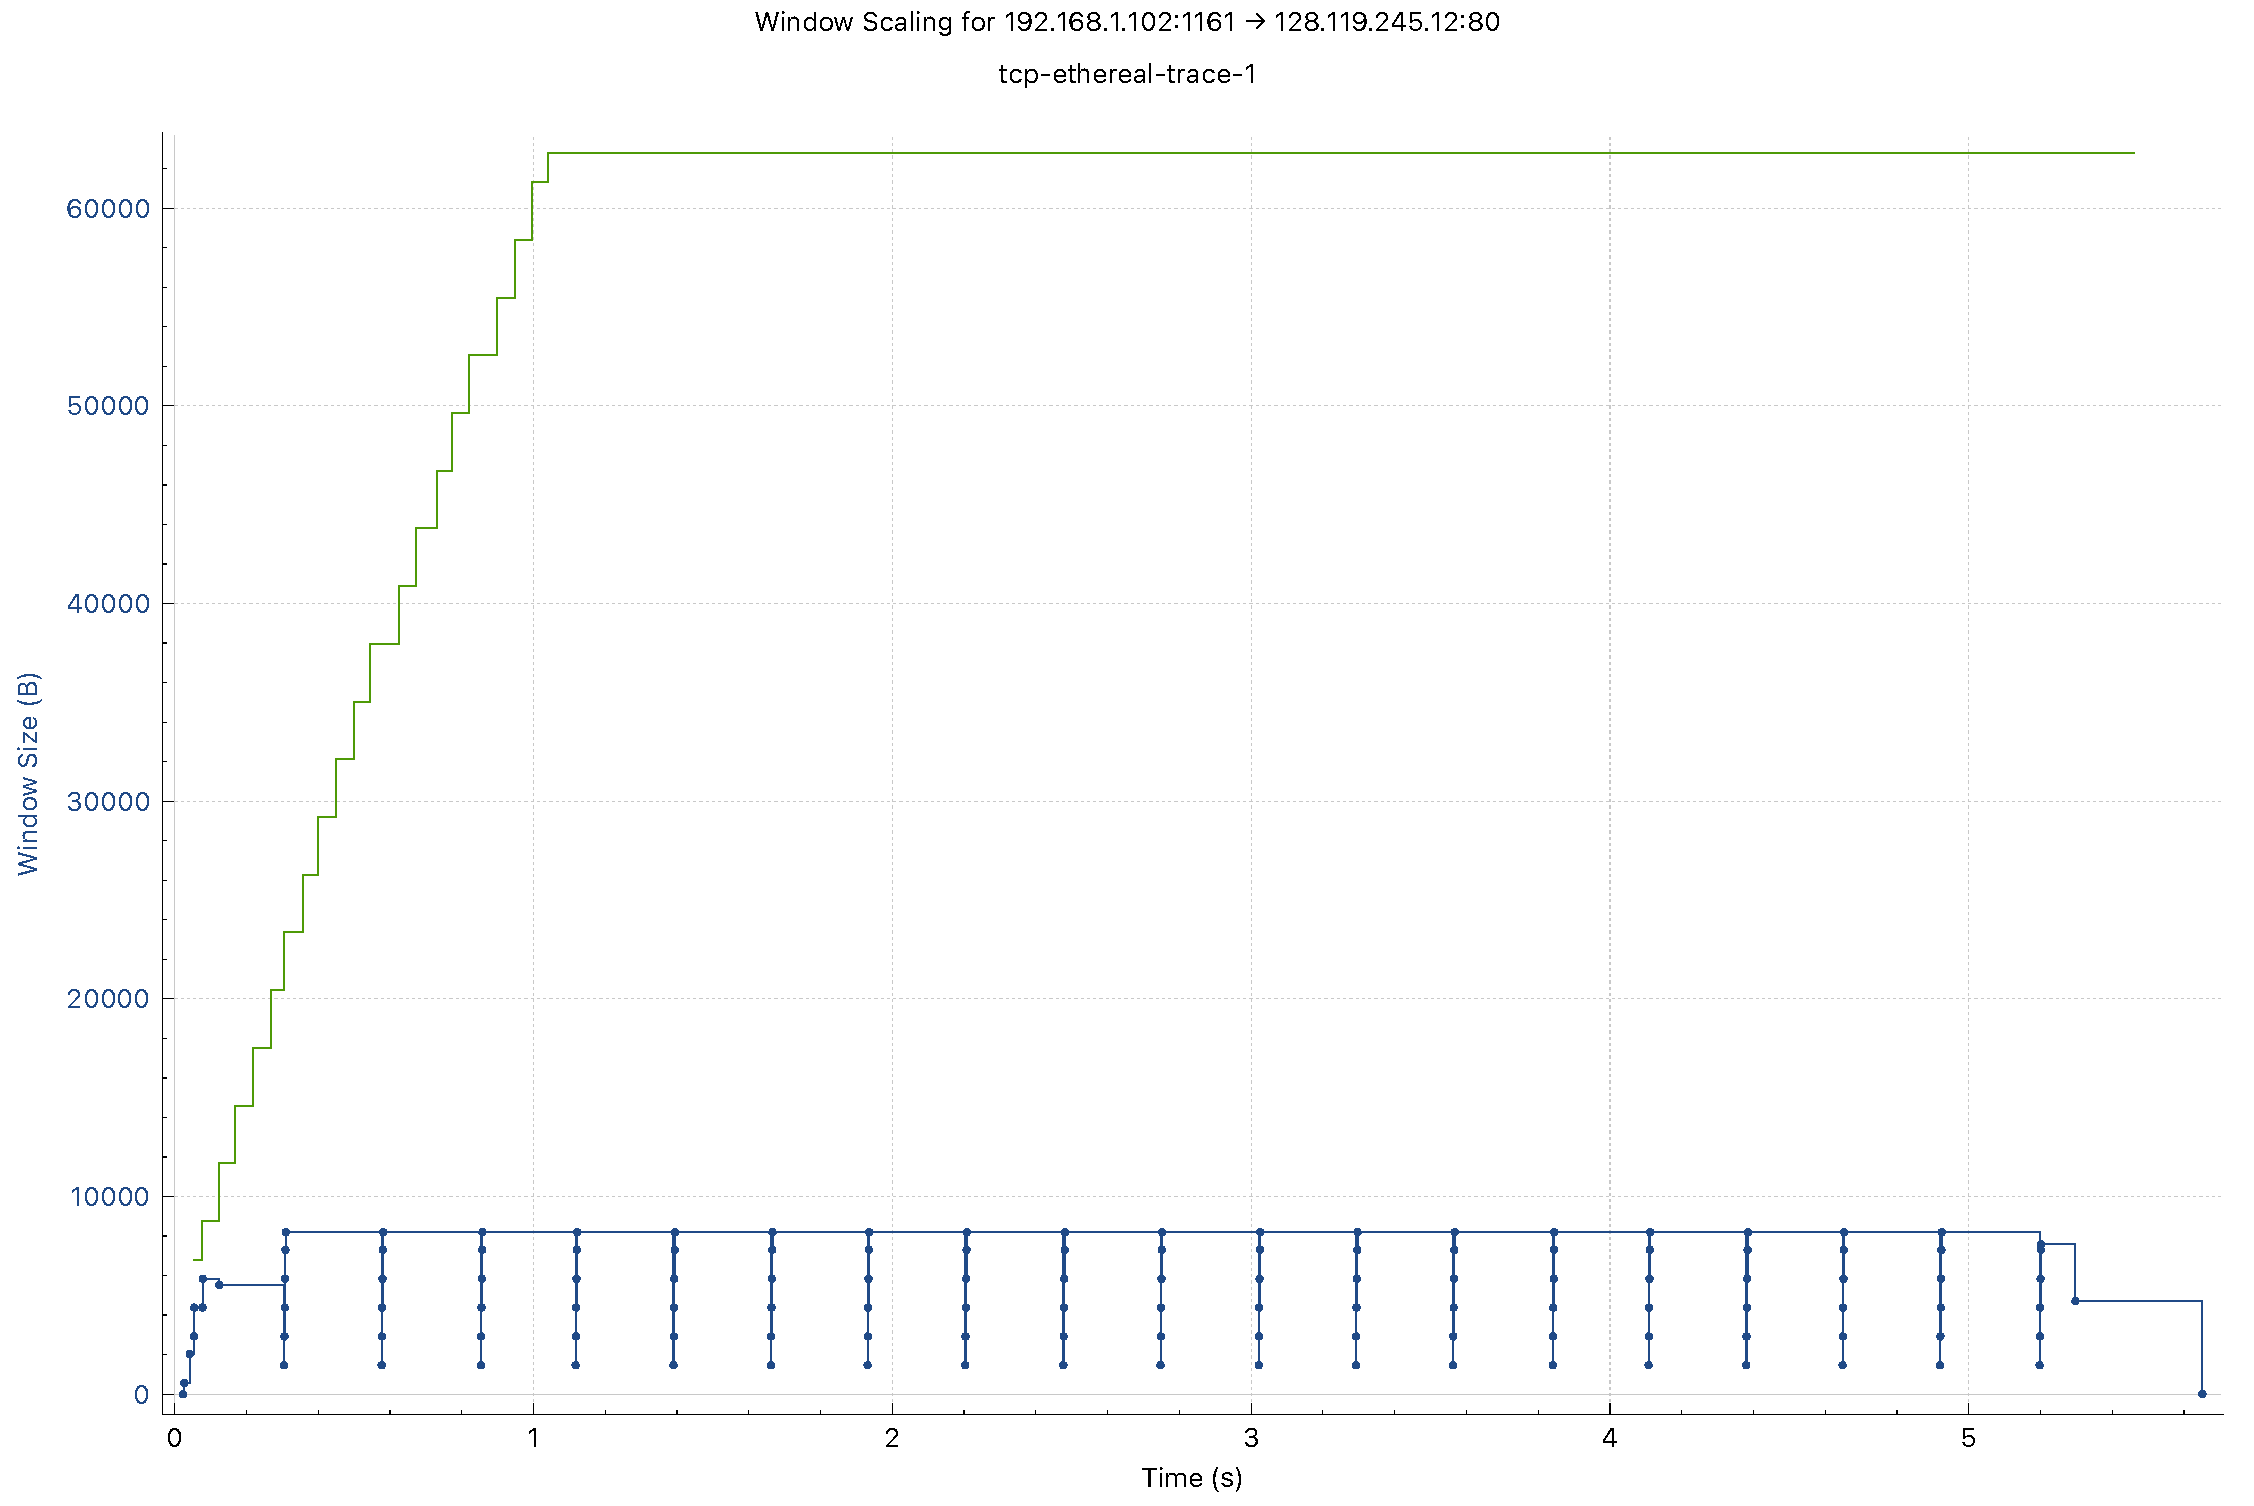
\includegraphics[width=0.49\linewidth]{img/tcp-ethereal-trace-window-scaling.pdf}
        \caption{Time Sequence (Stevens) (left) and Window Scaling (right) graph in the direction from the client to the HTTP server plotted by Wireshark for the entire TCP connection in tcp-ethereal-trace-1.}
        \label{fig:tcp-ethereal-trace}
    \end{figure}

    \item For our own collected traces, the whole TCP connection happened in the slow start phase and never entered the congestion avoidance phase, as shown in the Time / Sequence (Stevens) graph in Figure~\ref{fig:our-traces}. Our behaviors differ from those discussed in the textbook in that the initial window size is set to 10 MSS as suggested in RFC 6928, instead of just 1 MSS.
\end{enumerate}

\section{Conclusion}

From the lab, I've learned that TCP implementation can deviate from the standard in a significant way. For example, although the initial window size is defined to be around 4 segments in RFC 3390, the practice is that the initial window size is set to 10 MSS as suggested in the experimental RFC 6928 and has even become a user-tunable parameter e.g., \texttt{ip route replace initcwnd}.

The Wireshark interface contains some surprises. The sequence number displayed for each packet is \emph{relative} by default, with the first segment has a sequence number of 0. The default sending direction for ``TCP Stream Graphs'' is the one from the other end to the device running Wireshark, rendering the graphs quite useless on first sight as there were relatively few traffic (and thus data points on the graphs) in this direction when we were uploading a file.

\end{document}
